
\subsection{Strongly monotonic measurable semiring}
\label{sec:strongly_monotonic_measurable_semiring}
A commutative semiring is an algebraic structure (see~\cite{bruggink2015proving}\cite{endrullis2024generalized_arxiv_v2}). In this work, we adapt the concept of an ordered semiring from~\cite{endrullis2024generalized_arxiv_v2}. 
The key difference is that the semiring is required to be equipped with a homomorphism to the extended real numbers instead of being well-founded.
Throughout the remainder of this article, $<$ and $\leq$ denote the canonical irreflexive and reflexive orders on the set of extended real numbers $\overline{\mathbb{R}} = \mathbb{R} \cup \{-\infty, +\infty\}$.
\begin{definition}[Strongly monotonic measurable semiring]
    \label{def:real_strongly_monotonic_semiring}
    A \textbf{strongly monotonic measurable semiring} $(S, \oplus, \odot, 0, 1, \prec, \mu)$ consists of
    \begin{itemize} 
        \item A commutative semiring $(S, \oplus, \odot, 0, 1)$,
        \item A non-empty irreflexive order $\prec$ on $S$,
        \item A homomorphism $\mu : (S, \prec) \to ( \overline{\mathbb{R}}, < )$,
    \end{itemize}
    such that $0 \neq 1$ and for all $x,y,z,w \in S$, for all $\delta \in \mathbb{R}_{\geq 0}$, we have
        \begin{align*}
            1 \preceq x \land 1 \preceq y 
            &\Rightarrow
            1 \preceq x \oplus y
            &\tag{S0} \label{ax:s0} 
            \\ 
            x \preceq x' \land y \preceq y' 
            &\Rightarrow
            x \oplus y \preceq x' \oplus y'
            &\tag{S1} \label{ax:s1} 
            \\   
            % x < y  
            % &\Rightarrow
            % x \oplus z \leq y \oplus z 
            % \tag{S1} \label{eq:ordered_semiring_plus_monotonic} 
            % \\ w
            x \prec x' \land y \prec y'  
            &\Rightarrow
            x \oplus y \prec x' \oplus y'
            &\tag{S2} \label{ax:s2} 
            \\
            \delta + \mu(x) < \mu(y) \land \delta + \mu(z) < \mu(w)
            &\Rightarrow
            \delta + \mu(x \oplus z) < \mu(y \oplus w)
            &\tag{S3} \label{ax:s2'}
            \\
            x \preceq x'
            &\Rightarrow 
            x \odot y \preceq x' \odot y 
            &\tag{S4} \label{ax:s3} 
            \\
            x \prec x' \land y \neq 0 
            &\Rightarrow
            x \odot y \prec x' \odot y
            &\tag{S5} \label{ax:s4}
            \\ 
            \delta + \mu(x) < \mu(y) \land 1 \preceq z \neq 0
            &\Rightarrow
            \delta + \mu(x \odot z) < \mu(y \odot z)
            &\tag{S6} \label{ax:s4'}
            \\
            \delta+ \mu(x) < \mu(x') \land y \neq 0
            &\Rightarrow
            \mu(x \odot y) < \mu(x' \odot y)
            &\tag{S7} \label{ax:s4''}
        %    \\
            % \\
            % 1 \leq z \neq 0 \land X < Y  
            % &\Rightarrow
            % \exists \mu(x * z) < \mu( y * z)
            % \tag{S101} \label{eq:strongly_ordered_measurable_semiring_lt_preserved_neq0_geq1}  
        %      \\     
        %     a + X < Y \land z \neq 0 
        %    &\Rightarrow
        %    \exists b> 0. b + \mu(x* z) < \mu(y * z) 
        %    \tag{S3} \label{eq:ordered_semiring_times_stable_under_mesure} 
        \end{align*}
        where $\preceq$ denotes the reflexive closure of $\prec$. The semiring is a \textbf{strictly monotonic measurable semiring} if it additionally satisfies 
    \begin{flalign*}
        \hspace{4.5cm} x \prec x' 
        &\Rightarrow
        x \oplus y \prec x' \oplus y 
        &\tag{S8} \label{ax:s5} 
        \\
        \delta + \mu(x) < \mu(x')
        &\Rightarrow
        \delta + \mu(x \oplus y) < \mu(x' \oplus y)
        &\tag{S9} \label{ax:s5'}
    \end{flalign*}
\end{definition} 
\begin{example} 
    % The real tropical semiring $\mathfrak{T}' = (\mathbb{R} \cup \{+\infty\}, \min,+,+\infty, 0_\mathbb{R},<,\operatorname{id}_{\mathbb{R} \cup \{+\infty\}})$ has domain $\mathbb{R} \cup \{+\infty\}$, the binary function symbol $\oplus$ interpreted by $\min$ and the binary function symbol $\odot$ interpreted by $+$, the constant symbols $0_s$ and $1_s$ interpreted by $+\infty$ and $0_\mathbb{R}$, respectively, the binary relation symbol $\prec$ interpreted by the canonical order $<$ on $\mathbb{R} \cup \{+\infty\}$, and the unary function symbol $\mu$ interpreted by the identity function on $\mathbb{R} \cup \{+\infty\}$. The real tropical semiring is a strongly monotonic measurable semiring. It is not strictly monotonic measurable because $2 < 3$ but $2 \oplus 2 = \min(2,2) = 2 \not < 2 = \min(3,2) = 3 \oplus 2$.

     The real tropical semiring $\mathfrak{T}' = (\mathbb{R} \cup \{+\infty\}, \min,+_\mathbb{R},+\infty, 0_\mathbb{R},<_\mathbb{R},\operatorname{id}_{\mathbb{R} \cup \{+\infty\}})$ is an instance of the strongly monotonic measurable semiring where
     \begin{flalign*}
         S & \mapsto \mathbb{R} \cup \{+\infty\}
         \\
         \oplus & \mapsto \min
         \\
         \odot & \mapsto +_\mathbb{R}
         \\
         0_s & \mapsto +\infty
         \\
         1_s & \mapsto 0_\mathbb{R}
         \\
         \prec & \mapsto <_\mathbb{R}
         \\
         \mu & \mapsto \operatorname{id}_{\mathbb{R} \cup \{+\infty\}}
     \end{flalign*}

    It is a strongly monotonic measurable semiring but not strictly monotonic measurable, because we have $2 <_\mathbb{R} 3$ but $2 \oplus 2 = \min(2,2) = 2 \not <_\mathbb{R} 2 = \min(3,2) = 3 \oplus 2$.
\end{example}
\begin{example}
    % The real arctic semiring $\mathfrak{A}' = (\mathbb{R} \cup \{-\infty\},\max,+,-\infty, 0_\mathbb{R},<,\operatorname{id}_{\mathbb{R} \cup \{-\infty\}})$ has domain $\mathbb{R} \cup \{-\infty\}$, the binary function symbol $\oplus$ interpreted by $\max$ and the binary function symbol $\odot$ interpreted by $+$, the constant symbols $0_s$ and $1_s$ interpreted by $-\infty$ and $0_\mathbb{R}$, respectively, the binary relation symbol $\prec$ interpreted by the canonical order $<$ on $\mathbb{R} \cup \{-\infty\}$, and the unary function symbol $\mu$ interpreted by the identity function on $\mathbb{R} \cup \{-\infty\}$. The real arctic semiring is a strongly monotonic measurable semiring. It is not strictly monotonic measurable because $2 < 3$ but $2 \oplus 3 = \max(2,3) = 3 \not < 3 = \max(3,3) = 3 \oplus 3$.
    The real arctic semiring $\mathfrak{A}' = (\mathbb{R} \cup \{-\infty\},\max,+_\mathbb{R},-\infty, 0_\mathbb{R},<_\mathbb{R},\operatorname{id}_{\mathbb{R} \cup \{-\infty\}})$ is an instance of the strongly monotonic measurable semiring where
    \begin{flalign*}
        S & \mapsto \mathbb{R} \cup \{-\infty\}
        \\
        \oplus & \mapsto \max
        \\
        \odot & \mapsto +_\mathbb{R}
        \\
        0_s & \mapsto -\infty
        \\
        1_s & \mapsto 0_\mathbb{R}
        \\
        \prec & \mapsto <_\mathbb{R}
        \\
        \mu & \mapsto \operatorname{id}_{\mathbb{R} \cup \{-\infty\}}
    \end{flalign*}
    It is a strongly monotonic measurable semiring but not strictly monotonic measurable, because $2 <_\mathbb{R} 3$ but $2 \oplus 3 = \max(2,3) = 3 \not <_\mathbb{R} 3 = \max(3,3) = 3 \oplus 3$.
%    The real arctic semiring: $\mathfrak{A}' = (\mathbb{R} \cup \{-\infty\},\max,+,-\infty, 0,<,\operatorname{id}_{\mathbb{R} \cup \{-\infty\}})$.
\end{example}
\begin{example}
    The real arithmetic semiring $\mathfrak{N}' = (\mathbb{R}^+,+_\mathbb{R},*_\mathbb{R},0_\mathbb{R},1_\mathbb{R},<,\operatorname{id}_{\mathbb{R}^+})$ is an instance of the strongly monotonic measurable semiring where
    \begin{flalign*}
        S & \mapsto \mathbb{R}^+
        \\
        \oplus & \mapsto +_\mathbb{R}
        \\
        \odot & \mapsto *_\mathbb{R}
        \\
        0_s & \mapsto 0_\mathbb{R}
        \\
        1_s & \mapsto 1_\mathbb{R}
        \\
        \prec & \mapsto <_\mathbb{R}
        \\
        \mu & \mapsto \operatorname{id}_{\mathbb{R}^+}
    \end{flalign*}
    It is a strictly monotonic measurable semiring. 
    % The real arithmetic semiring $\mathfrak{N}' = (\mathbb{R}^+,+,*,0_\mathbb{R},1_\mathbb{R},<,\operatorname{id}_{\mathbb{R}^+})$ has as domain the set $\mathbb{R}^+$ of positive real numbers, the binary function symbol $\oplus$ interpreted by $+$ and the binary function symbol $\odot$ interpreted by $*$, the constant symbols $0_s$ and $1_s$ interpreted by $0_\mathbb{R}$ and $1_\mathbb{R}$, respectively, the binary relation symbol $\prec$ interpreted by the canonical order $<$ on $\mathbb{R}^+$, and the unary function symbol $\mu$ interpreted by the identity function on $\mathbb{R}^+$. The real arithmetic semiring is a strictly monotonic measurable semiring. 
\end{example}
\begin{example} 
    \label{example:real_semirings}
    The natural tropical semiring $\mathfrak{T} = (\mathbb{N} \cup \{+\infty\},\min,+_{\mathbb{N}},+\infty, 0_\mathbb{N}, <_{\mathbb{N}} , \operatorname{id}_{\mathbb{N} \cup \{+\infty\}})$ is an instance of the strongly monotonic measurable semiring where
    \begin{flalign*}
        S & \mapsto \mathbb{N} \cup \{+\infty\}
        \\
        \oplus & \mapsto \min
        \\
        \odot & \mapsto +_\mathbb{N}
        \\
        0_s & \mapsto +\infty
        \\
        1_s & \mapsto 0_\mathbb{N}
        \\
        \prec & \mapsto <_\mathbb{N}
        \\
        \mu & \mapsto \operatorname{id}_{\mathbb{N} \cup \{+\infty\}}
    \end{flalign*}
    The natural arctic semiring $\mathfrak{A} = (\mathbb{N} \cup \{-\infty\},\max,+_{\mathbb{N}},-\infty, 0_\mathbb{N},<_{\mathbb{N}}, \operatorname{id}_{\mathbb{N} \cup \{-\infty\}})$ is an instance of the strongly monotonic measurable semiring where
    \begin{flalign*}
        S & \mapsto \mathbb{N} \cup \{-\infty\}
        \\
        \oplus & \mapsto \max
        \\
        \odot & \mapsto +_\mathbb{N}
        \\
        0_s & \mapsto -\infty
        \\
        1_s & \mapsto 0_\mathbb{N}
        \\
        \prec & \mapsto <_\mathbb{N}
        \\
        \mu & \mapsto \operatorname{id}_{\mathbb{N} \cup \{-\infty\}}
    \end{flalign*}  
    The natural arithmetic semiring $\mathfrak{N} = (\mathbb{N},+_\mathbb{N},*,0_\mathbb{N},1_\mathbb{N},<_\mathbb{N},\operatorname{id}_\mathbb{N})$ is an instance of the strictly monotonic measurable semiring where
    \begin{flalign*}
        S & \mapsto \mathbb{N}
        \\
        \oplus & \mapsto +_\mathbb{N}
        \\
        \odot & \mapsto *_\mathbb{N}
        \\
        0_s & \mapsto 0_\mathbb{N}
        \\
        1_s & \mapsto 1_\mathbb{N}
        \\
        \prec & \mapsto <_\mathbb{N}
        \\
        \mu & \mapsto \operatorname{id}_\mathbb{N}
    \end{flalign*}
\end{example}

% \begin{notation} 
%     \label{def:bigodot}
% Let $(S, \oplus, \odot, 0_s, 1_s)$ be a semiring. We extend naturally the binary operations $\oplus$ and $\odot$ to finite sets $E \subseteq S$ by letting
%     \begin{itemize}
%         \item $\bigodot \emptyset \overset{\operatorname{def}}{=} 1_s$ and $\bigodot \left( E \cup \{x\} \right) \overset{\operatorname{def}}{=} \left( \bigodot E \right) \odot x$;
%         \item $\bigoplus \emptyset \overset{\operatorname{def}}{=} 0_s$ and $\bigoplus \left( E \cup \{x\} \right) \overset{\operatorname{def}}{=} \left( \bigoplus E \right) \oplus x$.
%     \end{itemize}
% %  \begin{flalign*}
% %     \bigodot \emptyset &\overset{\operatorname{def}}{=} 1_s
% % \\
% %     \bigodot \left( E \cup \{x\} \right) &\overset{\operatorname{def}}{=} \left( \bigodot E \right) \odot x
% %     \\
% %     \bigoplus \emptyset &\overset{\operatorname{def}}{=} 0_s
% %     \\
% %         \bigoplus \left( E \cup \{x\} \right) &\overset{\operatorname{def}}{=} \left( \bigoplus E \right) \oplus x
% % \end{flalign*}
% \end{notation}

% \textcolor{blue}{\begin{remark}
%     \label{remark:diff_measurable_semiring}
% A strongly monotonic measurable semiring differs from a well-founded strongly monotonic semiring in~\cite{endrullis2024generalized} in four ways:
% \begin{enumerate}[label=(\arabic*),noitemsep]
%     \item Replacing well-foundedness with the homomorphism~$\mu$ and introducing Axioms \eqref{ax:s2'}, \eqref{ax:s4'}, and \eqref{ax:s4''}. This modification enables the use of non-well-founded semirings (e.g., as in~\autoref{example:real_semirings}).
%     % \item Removing the condition $1_S \preceq y$ from the original Axioms~(S3) and~(S4)\todo{This is not helpful}, resulting in our Axioms~(S4) and~(S5). This relaxation allows inclusion of elements smaller than $1_S$, as motivated in~\autoref{remark:greater_than_1}.
%     \item Adding Axiom~\eqref{ax:s0}. This technical adjustment ensures that if every $\mathcal{T}$-valued element of a type graph (see~\autoref{def:weighted_type_graph}) has a weight greater than $1_S$, then all objects subject to rewriting inherit this property.
%     \item Defining $\preceq$ as the reflexive closure of $\prec$ to simplify the theory. This is motivated by the fact that concrete semirings proposed in prior work and our paper satisfy this property.
% \end{enumerate} 
% \end{remark}}
\subsection{Measuring objects by counting morphisms}
\begin{example}
    \label{example:weighted_type_graph}
     In \textbf{Graph}, the weighted type graph $\mathcal{T} = (T, \mathbb{E}, \mathcal{S}, w)$ with $\mathcal{S}$ as the real arithmetic semiring $(\mathbb{R}^+, +, *, 0_\mathbb{R}, 1_\mathbb{R}, <, \operatorname{id}_{\mathbb{R}^+})$,
     $T$ as the graph illustrated below (without superscripts), $\mathbb{E}=\{e_{11a},e_{12a},e_{21a},e_{11b}\}$ as the set of morphism-rulers where 
     $e_{uvl}$ has domain 
     \tikz[baseline=-0.5ex]{
        \node (x) at (0,0) {$\bullet$};
        \node (y) at (1,0) {$\bullet$};
        \draw[->] (x) -- (y) node[midway, above] {$l$};
    } and image 
    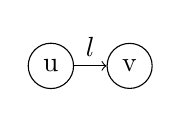
\begin{tikzpicture}
        \node[draw, circle] (x) at (0,0) {$\mathrm{u}$};
        \node[draw, circle] (y) at (1,0) {$\mathrm{v}$};
        \draw[->]  (x) -- (y) node [midway,above] {$l$};
    \end{tikzpicture} in the graph $T$,
    and $w(e) = 1.0$ for all $e \in \mathbb{E}$, can be visualized as follows:
    \begin{center}
        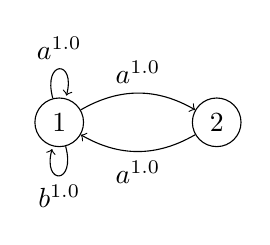
\begin{tikzpicture}
            \graphbox{}{0mm}{0mm}{32mm}{28mm}{-10mm}{-14mm}{
                \node[draw,circle] (1) at (0,0) {1};
                \node[draw,circle] (2) at (2,0) {2};
                \draw[->] (1) edge[loop above] node[midway, above] {$a^{1.0}$} (1) ;
                \draw[->] (1) edge[loop below] node[midway, below] {$b^{1.0}$} (1) ;
                \draw[->] (1) edge[bend left] node[midway, above] {$a^{1.0}$}  (2)  ;
                \draw[->] (2) edge[bend left] node[midway, below] {$a^{1.0}$} (1)   ;
            }
        \end{tikzpicture}
    \end{center}
\end{example}

\begin{example}
    Consider the following morphisms and the weighted type graph $\mathcal{T}$ from \autoref{example:weighted_type_graph}:
    \begin{center}
        \resizebox{0.49\textwidth}{!}{
        \begin{tikzpicture}
          \graphbox{\( L \)}{-50mm}{0mm}{40mm}{39mm}{2mm}{-6mm}{
            \coordinate (o) at (0mm,-10mm); 
            \node[draw,circle] (l1) at ($(o)+(-10mm,0mm)$) {1};
            \node[draw,circle] (l2) at ($(l1)+(2,0)$) {2};
            \node[draw,circle] (l3) at ($(l1) + (1,0)$) {3};
            \draw[] (l1) -- (l3) node[midway,above] {a};
            \draw[] (l3) -- (l2) node[midway,above] {a};
        } 
            \graphbox{$T$}{0mm}{0mm}{40mm}{39mm}{-10mm}{-17mm}{
                \node[draw,circle] (1) at (0,0) {$1\ 2$};
                \node[draw,circle] (2) at (2,0) {3};
                \draw[->] (1) edge[loop above] node[midway, above] {$a^{1.0}$} (1) ;
                \draw[->] (1) edge[loop below] node[midway, below] {$b^{1.0}$} (1) ;
                \draw[->] (1) edge[bend left] node[midway, above] {$a^{1.0}$}  (2)  ;
                \draw[->] (2) edge[bend left] node[midway, below] {$a^{1.0}$} (1)   ;
            }
            \node () at (-5mm,-15mm) {$\overset{h_{11}^1}{\to}$};
        \end{tikzpicture}
        }
        \resizebox{0.49\textwidth}{!}{
            \begin{tikzpicture}
              \graphbox{\(L\)}{-50mm}{0mm}{40mm}{39mm}{2mm}{-6mm}{
                \coordinate (o) at (0mm,-10mm); 
                \node[draw,circle] (l1) at ($(o)+(-10mm,0mm)$) {1};
                \node[draw,circle] (l2) at ($(l1)+(2,0)$) {2};
                \node[draw,circle] (l3) at ($(l1) + (1,0)$) {3};
                \draw[] (l1) -- (l3) node[midway,above] {a};
                \draw[] (l3) -- (l2) node[midway,above] {a};
            } 
                \graphbox{$T$}{0mm}{0mm}{40mm}{39mm}{-10mm}{-19mm}{
                    \node[draw,circle] (1) at (0,0) {$1\ 2\ 3$};
                    \node[draw,circle] (2) at (2,0) {};
                    \draw[->] (1) edge[loop above] node[midway, above] {$a^{1.0}$} (1) ;
                    \draw[->] (1) edge[loop below] node[midway, below] {$b^{1.0}$} (1) ;
                    \draw[->] (1) edge[bend left] node[midway, above] {$a^{1.0}$}  (2)  ;
                    \draw[->] (2) edge[bend left] node[midway, below] {$a^{1.0}$} (1)   ;(1)   ;
                }
                \node () at (-5mm,-15mm) {$\overset{h_{11}^2}{\to}$};
            \end{tikzpicture}
            }
      \end{center}
    We have $ w_\mathcal{T}(h_{11}^1) = w(e_{13a})^{m_{e_{13a}}(h_{11}^1)} \odot w(e_{31a})^{m_{e_{31a}}(h_{11}^1)} =
     1.0^1 * 1.0^1 = 1.0$ and $
        w_\mathcal{T}(h_{11}^2) 
        % = 1.0^1 * 1.0^1 
        = 1.0$
\end{example}

\subsection{Estimating weights of pushout objects}
Let \( \mathcal{R} = \mathcal{A} \cup \mathcal{B} \) be a set of DPO rewriting rules and let \(\mathcal{T} = (T, \mathbb{E}, \mathcal{S}, w)\) be a weighted type graph over the strongly monotonic measurable semiring $\mathcal{S}$.

The following proposition ensures that every morphism to a type graph $(T,S,\mathbb{E}, w)$ has a weight different from $0_S$ and greater than or equal to $1_S$.
%  then the weight of a morphism to a type graph is greater than $1_S$ too. 
This lemma will be used in \autoref{thm:termination_grs}.
\begin{proposition}  
    \label{prop_endrullis_2d7}
    Let $(S, \oplus, \odot, 0_S, 1_S, \prec, \mu)$ be a strongly monotonic measurable semiring. We have for all $x,y\in S$:
    \begin{align*}
        0_S \neq x \land 0_S \neq y 
        &\Rightarrow 0_S \neq x \odot y 
        \tag{S10} \label{eq:prop_neq0_mul_neq0}  
        \\
        1_S \preceq x \land 1_S \preceq y \land 0_S \neq x \land 0_S \neq y  
        &\Rightarrow
         1_S \preceq x \odot y 
         \tag{S11} \label{eq:prop_neg0_ge1_mul_ge1}  
         \\
         0_S \neq x \land 0_S \neq y   
         &\Rightarrow 0_S \neq x \oplus y
         \tag{S12} \label{eq:prop_neq0_plus_neq0}  
    \end{align*}
\end{proposition}

\begin{proof}
    \label{proof_prop_endrullis_2d7}
    Let $x,y \in S$ such that $x, y \neq 0_S$. By definition, $\prec$ is not empty, therefore there exist $a, b \in S$ such that $a \prec b$.
    \begin{itemize}
        \item $\prec$ is irreflexive, because $\mu: (S, \prec) \to (\overline{\mathbb{R}}, <)$ is a homomorphism.
        \item \ref*{eq:prop_neq0_mul_neq0}:  
        Suppose $(x \odot y)=0_S$. 
        We have 
        \begin{flalign*}
             0_S &= a \odot 0_S & \text{$0_S$ is annihilator for $\odot$}\\
                 &= a \odot (x \odot y) &\text{by assumption on $x \odot y$}\\ 
                 &= a \odot x \odot y &\text{by associativity} \\
                 &\prec b \odot x \odot y &\text{by \eqref{ax:s4} and $x,y\neq 0_S$}\\
                 &= b \odot (x \odot y)  &\text{by associativity}  \\
                 &= b \odot 0_S &\text{by assumption on $x \odot y$} \\
                 &= 0_S
        \end{flalign*}
         which contradicts the irreflexivity of $\prec$. 
        \item \ref*{eq:prop_neg0_ge1_mul_ge1}:
        Suppose
          $1_S \preceq x$ and $1_S \preceq y$. We have either $1_S = x$ or $1_S \prec x$. If $1_S = x$ then 
          \begin{flalign*}
            x \odot y &= 1_S \odot y & \\
                      &= y  & \\
                      & \succeq 1_S &\text{by assumption}
          \end{flalign*}
          If $1_S \prec x$ then $
        %   1_S \preceq y = 
          1_S \odot y \prec x \odot y$ by \eqref{ax:s4} since $y \neq 0$ by assumption.
        \item \ref*{eq:prop_neq0_plus_neq0}:  
        By \eqref{ax:s4}, we have $a \odot x \prec b \odot x$ and $a\odot y \prec b \odot y $. 
        \begin{flalign*}
            a \odot \left(x  \oplus y \right) &= \left( a \odot x \right)  \oplus \big(a \odot y \big)  & \text{by distributivity}\\
            & \prec \left(b \odot x \right)   \oplus \left( b \odot y \right)  & \text{by \eqref{ax:s2}\newline}\\
            & = b \odot \left(x  \oplus y \right) & \text{by distributivity}
        \end{flalign*} 
        if $x  \oplus y = 0_S$ then we have $0_S = a \odot 0_S = a \odot \left(x  \oplus y\right) \prec b \odot \left(x  \oplus y\right) = b \odot 0_S = 0_S$ which contradicts the irreflexivity of $\prec$. 
    \end{itemize}
\end{proof} 

% \begin{proposition}  
%     % Let $\mathcal{S} = (S, \oplus, \odot, 0_\mathcal{S}, 1_\mathcal{S}, \prec, \mu)$ be a strongly monotonic measurable semiring. We have 
%     For all $x,y$ in $\mathcal{S}$:
%     \begin{align*}
%         0_\mathcal{S} \neq x \land 0_\mathcal{S} \neq y 
%         &\Rightarrow 0_\mathcal{S} \neq x \odot y 
%         \\
%         1_\mathcal{S} \preceq x \land 1_\mathcal{S} \preceq y \land 0_\mathcal{S} \neq x \land 0_\mathcal{S} \neq y  
%         &\Rightarrow
%          1_\mathcal{S} \preceq x \odot y 
%          \\
%          0_\mathcal{S} \neq x \land 0_\mathcal{S} \neq y   
%          &\Rightarrow 0_\mathcal{S} \neq x \oplus y
%     \end{align*}
% \end{proposition}

    Suppose that for all $x \in \mathcal{S}$, if $ 1_\mathcal{S} \preceq x \neq 0_\mathcal{S}$ then $\mu(x) \geq \mu(1_\mathcal{S})$ and $\mu(x) \in \mathbb{R}$. 
    By definition of a weighted type graph, $1_\mathcal{S} \leq w(e)\neq 0_\mathcal{S}$ for all $e\in\mathbb{E}$.
    Therefore, by the proposition above and the definition of the weight of a morphism (\autoref{def:weight_of_a_morphism_relative_to_a_type_graph}), for all morphisms \( h \) from a finite graph $G$ to $\mathcal{T}$, we have \( 0_\mathcal{S} \neq w_\mathcal{T}(h) \succeq 1_\mathcal{S} \). 
    By the above proposition, Axiom \eqref{ax:s0} and the definition of the weight of an object (\autoref{def:weight_of_an_object_relative_to_a_type_graph}), we conclude that for all objects \( G \) with $\operatorname{Hom}(G,T)\neq \emptyset$, \( 0_\mathcal{S} \neq w_\mathcal{T}(G) \succeq 1_\mathcal{S} \). By assumption, we have that for all objects \( G \) with $\operatorname{Hom}(G,T)\neq \emptyset$, \( \mu(w_\mathcal{T}(G)) \geq \mu(1_\mathcal{S}) = 0 \) if $\mathcal{S}$ is the real tropical or arctic semiring, and \( \mu(w_\mathcal{T}(G)) \geq 1 \) if $\mathcal{S}$ is the arithmetic semiring.

Suppose additionally that for every graph $G$ subject to rewriting, we have $\operatorname{Hom}(G,T)\neq \emptyset$. The rewriting relation \( \Rightarrow_{\mathcal{A},\mathfrak{F}} \) is terminating relative to $\Rightarrow_{\mathcal{B},\mathfrak{F}}$ if there exists a constant $\delta > 0$ such that: (i) for all \(G \Rightarrow_{\mathcal{A},\mathfrak{F}} H\), \( \mu(w_\mathcal{T}(G)) > \mu(w_\mathcal{T}(H)) + \delta \), and (ii) for all \(G \Rightarrow_{\mathcal{B},\mathfrak{F}} H\), \( \mu(w_\mathcal{T}(G)) \geq \mu(w_\mathcal{T}(H)) \). However, directly verifying all rewriting steps is infeasible due to the potentially infinite number of rewriting steps.


\noindent
\begin{minipage}{0.7\textwidth}\setlength{\parindent}{1em}
    Consider a DPO diagram (illustrated on the right) that defines a rewriting step \( G \Rightarrow_{\rho,\mathfrak{F}} H \). 
    If the left pushout square is weighable with $\mathcal{T}$ and the right pushout square is bounded above by $\mathcal{T}$ (concepts defined in \autoref{def:weighable}), then, by \cite[Lemma 4.13]{endrullis2024generalized_arxiv_v2}, we obtain:
\end{minipage}%
\hfill
\begin{minipage}{0.29\textwidth}
    \hfill
    \resizebox{0.85\textwidth}{!}{
    \begin{tikzpicture}
        % [node distance=11mm]
        \node (I) at (0,0) {$K$};
        \node (L) at (-2,0) {$L$};
        \node (R) at (2,0) {$R$};
        \node (G) at (-2,-2) {$G$};
        \node (C) at (0,-2) {$C$};
        \node (H) at (2,-2) {$H$};
        \draw [->] (I) to  node [midway,below] {$l$} (L);
        \draw [->] (I) to  node [midway,below] {$r$} (R);
        \draw [->] (L) to node [midway,right] {$m$} (G);
        \draw [->] (I) to node [midway,right] {$u$} (C);
        \draw [->] (R) to node [midway,left] {$m'$} (H);
        \draw [->] (C) to node [midway,above] {$l'$} (G);
        \draw [->] (C) to node [midway,above] {$r'$} (H);
        \node [at=($(I)!.5!(G)$)] {\normalfont PO};
        \node [at=($(I)!.5!(H)$)] {\normalfont PO};
      \end{tikzpicture}
    }
\end{minipage}

% \begin{flalign*}
%     w_\mathcal{T}(G) 
%         & \overset{def}{=} \bigoplus_{t_G: G \rightarrow T} w_\mathcal{T}(t_G) 
%         \overset{def}{=} \bigoplus_{t_K: K \rightarrow T} \bigoplus_{\substack{t_G: G \rightarrow T\\ t_K = l \star m \star t_G}} w_\mathcal{T}(t_G) \\
%     w_\mathcal{T}(H) 
%         &\overset{def}{=} \bigoplus_{t_H: H \rightarrow T} w_\mathcal{T}(t_H) 
%          \overset{def}{=} \bigoplus_{t_K: K \rightarrow T} \bigoplus_{\substack{t_H: H \rightarrow T\\ t_K = r \star m' \star t_H}} w_\mathcal{T}(t_H)
% \end{flalign*}

% If the left pushout square is weighable with $\mathcal{T}$ and the right pushout square is bounded above by $\mathcal{T}$ (concepts defined in \autoref{def:weighable}), then, by \cite[Lemma 5.10]{endrullis2024generalized_lmcs}, we derive the following assertions:
% \begin{flalign*}
%     w_\mathcal{T}(G) 
%         & = \bigoplus_{t_K: K \rightarrow T} \bigoplus_{\substack{t_G: G \rightarrow T\\ t_K = l \star m \star t_G}} w_\mathcal{T}(m \star t_G) \odot (l' \star t_G - u) \\
%     w_\mathcal{T}(H) 
%         &  \preceq \bigoplus_{t_K: K \rightarrow T} \bigoplus_{\substack{t_H: H \rightarrow T\\ t_K = r \star m' \star t_H}} w_\mathcal{T}(m' \star t_H) \odot (r' \star t_H - u)
% \end{flalign*}
% By \cite[Theorem 5.12]{endrullis2024generalized_lmcs}, it follows:
% \begin{flalign*}
%     w_\mathcal{T}(G) 
%         & = \bigoplus_{t_K: K \rightarrow T} 
%         \bigoplus_{\substack{t_C: C \rightarrow T\\ t_K = u \star t_C}}
%         \bigoplus_{\substack{t_L: L \rightarrow T\\ t_K = l \star t_L}}
%             w_\mathcal{T}(t_L) \odot w_\mathcal{T}(t_C - u) \\
%     w_\mathcal{T}(H) 
%         &  \preceq \bigoplus_{t_K: K \rightarrow T} 
%         \bigoplus_{\substack{t_C: C \rightarrow T\\ t_K = u \star t_C}}
%         \bigoplus_{\substack{t_R: R \rightarrow T\\ t_K = r \star t_R}}
%             w_\mathcal{T}(t_R) \odot w_\mathcal{T}(t_C - u) \\
% \end{flalign*}
% By \cite[Theorem 5.13]{endrullis2024generalized_lmcs}, we have the following assertions: 
\begin{flalign*}
    w_\mathcal{T}(G) 
        & = \bigoplus_{t_K: K \rightarrow T} 
        \left ( \bigoplus_{\substack{t_C: C \rightarrow T\\ t_K = u \star t_C}}
          w_\mathcal{T}(t_C - u) \right ) 
          \odot
        \left (\bigoplus_{\substack{t_L: L \rightarrow T\\ t_K = l \star t_L}}
        w_\mathcal{T}(t_L) \right )
         \\
    w_\mathcal{T}(H) 
        &  \preceq \bigoplus_{t_K: K \rightarrow T} 
        \left ( \bigoplus_{\substack{t_C: C \rightarrow T\\ t_K = u \star t_C}}
         w_\mathcal{T}(t_C - u) \right ) 
         \odot 
         \left ( \bigoplus_{\substack{t_R: R \rightarrow T\\ t_K = r \star t_R}}
            w_\mathcal{T}(t_R) \right ) \\
\end{flalign*}
According to these results, a termination criterion will be established by comparing the weights 
$\bigoplus_{\substack{t_L: L \rightarrow T\\ t_K = l \star t_L}}
        w_\mathcal{T}(t_L)$ and 
$\bigoplus_{\substack{t_R: R \rightarrow T\\ t_K = r \star t_R}} 
        w_\mathcal{T}(t_R)$ for every $t_K: K \rightarrow T$.

\subsection{Decreasing rules}
\label{sec:nwf:decreasing_rules}
The definition below adapts the concept of decreasing rules from~\cite{endrullis2024generalized_arxiv_v2}. The difference lies in the treatment of weight comparisons for uniformly decreasing and closure decreasing rules: instead of directly comparing weights, we evaluate the difference between weights relative to the homomorphism $\mu$ of the strongly monotonic measurable semirings.
%  This difference must exceed a fixed positive constant $\delta \in \mathbb{R}_{>0}$.

\begin{definition}[Decreasing Rules]
    \label{def:nwf:decreasing_rule}
    Let $\mathcal{T} = (T,\mathbb{E}, (S, \oplus, \odot, 0_S, 1_S, \prec, \mu), w)$ be a finitary weighted type graph, \(\mathfrak{F}\) a DPO rewriting framework, $\rho = (L \overset{l}{\leftarrow} K \overset{r}{\rightarrow} R)$ a DPO rewriting rule, and $\delta \in \mathbb{R}_{>0}$. 

    \noindent
    The rule $\rho$ is \textbf{weakly decreasing} w.r.t. $\mathcal{T}$ in $\mathfrak{F}$ if 
            for every $t_K : K \to T$,
                $$ 
                  w_\mathcal{T}(\{l \star - = t_K\}) \succeq w_\mathcal{T}(\{r\star - = t_K\})$$
           
    \noindent
    The rule $\rho$ is \textbf{$\delta$-uniformly decreasing} w.r.t. $\mathcal{T}$ in $\mathfrak{F}$ if the following hold:
        \begin{itemize}
            \item[]- there exists a context closure $c_\rho$ for $\rho$ and $\mathcal{T}$ in $\mathfrak{F}$, 
            \item[]- for every $t_K : K \to T$,
            \begin{itemize}
                \item[] $\bullet$ $\{l \star - = t_K\} = \emptyset = \{r \star - = t_K\}$, or
                \item[] $\bullet$ $\mu(w_\mathcal{T}(\{l \star - = t_K\}))  >   \mu(w_\mathcal{T}(\{r \star - = t_K\})) + \delta$.
            \end{itemize}
        \end{itemize}  
         
    \noindent
    The rule $\rho$ is
            \textbf{$\delta$-closure decreasing} w.r.t. $\mathcal{T}$ in $\mathfrak{F}$ if the following hold:
            \begin{itemize}
                \item[]- $S$ is strictly monotonic measurable semiring,
                \item[]- $\rho$ is weakly decreasing,
                \item[]- there exists a context closure $c_\rho$ for $\rho$ and $\mathcal{T}$ in $\mathfrak{F}$,
                \item[]- $ \mu(w_\mathcal{T}(\{l \star - = t_K\}))  >  \mu(w_\mathcal{T}(\{r \star - = t_K\}))  + \delta$ for $t_K = l \star c_\rho$.
            \end{itemize}
\end{definition}

\begin{example}
    \label{example:nwf:decreasing_rule}
    Consider the DPO rule in \autoref{ex:grsaa} and the weighted type graph in \autoref{example:weighted_type_graph} over the real arithmetic semiring $\mathfrak{N}' = (\mathbb{R}^+,+,*,0_\mathbb{R},1_\mathbb{R},<,\operatorname{id}_{\mathbb{R}^+})$. There are $t_K^{11}, t_K^{12}, t_K^{21}, t_K^{22}:K \rightarrow T$ as depicted below:

    \begin{center}
        \resizebox{0.49\textwidth}{!}{
            \begin{tikzpicture}
            \graphbox{\( K \)}{-50mm}{0mm}{40mm}{30mm}{2mm}{-6mm}{
                \coordinate (o) at (0mm,-10mm); 
                \node[draw,circle] (l1) at ($(o)+(-10mm,0mm)$) {1};
                \node[draw,circle] (l2) at ($(l1)+(2,0)$) {2};
                % \node[draw,circle] (l3) at ($(l1) + (1,0)$) {3};
                % \draw[] (l1) -- (l3) node[midway,above] {a};
                % \draw[] (l3) -- (l2) node[midway,above] {a};
            } 
                \graphbox{$T$}{0mm}{0mm}{40mm}{30mm}{-10mm}{-15mm}{
                    \node[draw,circle] (1) at (0,0) {$1\ 2$};
                    \node[draw,circle] (2) at (2,0) {};
                    \draw[->] (1) edge[loop above] node[midway, above] {$a$} (1) ;
                    \draw[->] (1) edge[loop below] node[midway, below] {$b$} (1) ;
                    \draw[->] (1) edge[bend left] node[midway, above] {$a$}  (2)  ;
                    \draw[->] (2) edge[bend left] node[midway, below] {$a$} (1)   ;
                }
                \node () at (-5mm,-15mm) {$\overset{t_K^{11}}{\to}$};
            \end{tikzpicture}
            } 
            \resizebox{0.49\textwidth}{!}{
            \begin{tikzpicture}
                \graphbox{\( K \)}{-50mm}{0mm}{40mm}{30mm}{2mm}{-6mm}{
                \coordinate (o) at (0mm,-10mm); 
                \node[draw,circle] (l1) at ($(o)+(-10mm,0mm)$) {1};
                \node[draw,circle] (l2) at ($(l1)+(2,0)$) {2};
                % \node[draw,circle] (l3) at ($(l1) + (1,0)$) {3};
                % \draw[] (l1) -- (l3) node[midway,above] {a};
                % \draw[] (l3) -- (l2) node[midway,above] {a};
            } 
                \graphbox{$T$}{0mm}{0mm}{40mm}{30mm}{-10mm}{-15mm}{
                    \node[draw,circle] (1) at (0,0) {$1$};
                    \node[draw,circle] (2) at (2,0) {2};
                    \draw[->] (1) edge[loop above] node[midway, above] {$a$} (1) ;
                    \draw[->] (1) edge[loop below] node[midway, below] {$b$} (1) ;
                    \draw[->] (1) edge[bend left] node[midway, above] {$a$}  (2)  ;
                    \draw[->] (2) edge[bend left] node[midway, below] {$a$} (1)   ;
                }
                \node () at (-5mm,-15mm) {$\overset{t_K^{12}}{\to}$};
            \end{tikzpicture}
            }
            \hspace{5mm}
            
            \resizebox{0.49\textwidth}{!}{
            \begin{tikzpicture}
                \graphbox{\( K \)}{-50mm}{0mm}{40mm}{30mm}{2mm}{-6mm}{
                \coordinate (o) at (0mm,-10mm); 
                \node[draw,circle] (l1) at ($(o)+(-10mm,0mm)$) {1};
                \node[draw,circle] (l2) at ($(l1)+(2,0)$) {2};
                % \node[draw,circle] (l3) at ($(l1) + (1,0)$) {3};
                % \draw[] (l1) -- (l3) node[midway,above] {a};
                % \draw[] (l3) -- (l2) node[midway,above] {a};
            } 
                \graphbox{$T$}{0mm}{0mm}{40mm}{30mm}{-10mm}{-15mm}{
                    \node[draw,circle] (1) at (0,0) {2};
                    \node[draw,circle] (2) at (2,0) {1};
                    \draw[->] (1) edge[loop above] node[midway, above] {$a$} (1) ;
                    \draw[->] (1) edge[loop below] node[midway, below] {$b$} (1) ;
                    \draw[->] (1) edge[bend left] node[midway, above] {$a$}  (2)  ;
                    \draw[->] (2) edge[bend left] node[midway, below] {$a$} (1)   ;
                }
                \node () at (-5mm,-15mm) {$\overset{t_K^{21}}{\to}$};
            \end{tikzpicture}
            }
            \resizebox{0.49\textwidth}{!}{
            \begin{tikzpicture}
                \graphbox{\( K \)}{-50mm}{0mm}{40mm}{30mm}{2mm}{-6mm}{
                \coordinate (o) at (0mm,-10mm); 
                \node[draw,circle] (l1) at ($(o)+(-10mm,0mm)$) {1};
                \node[draw,circle] (l2) at ($(l1)+(2,0)$) {2};
                % \node[draw,circle] (l3) at ($(l1) + (1,0)$) {3};
                % \draw[] (l1) -- (l3) node[midway,above] {a};
                % \draw[] (l3) -- (l2) node[midway,above] {a};
            } 
                \graphbox{$T$}{0mm}{0mm}{40mm}{30mm}{-10mm}{-15mm}{
                    \node[draw,circle] (1) at (0,0) {};
                    \node[draw,circle] (2) at (2,0) {$1\ 2$};
                    \draw[->] (1) edge[loop above] node[midway, above] {$a$} (1) ;
                    \draw[->] (1) edge[loop below] node[midway, below] {$b$} (1) ;
                    \draw[->] (1) edge[bend left] node[midway, above] {$a$}  (2)  ;
                    \draw[->] (2) edge[bend left] node[midway, below] {$a$} (1)   ;
                }
                \node () at (-5mm,-15mm) {$\overset{t_K^{22}}{\to}$};
            \end{tikzpicture}
            }
      \end{center}
    The set $\{l \star - = t_K^{11}\}$ has two morphisms $h_{11}^1$ and $h_{11}^2$ as illustrated below:
    \begin{center}
        \resizebox{0.49\textwidth}{!}{
        \begin{tikzpicture}
          \graphbox{\( L \)}{-50mm}{0mm}{40mm}{40mm}{2mm}{-6mm}{
            \coordinate (o) at (0mm,-10mm); 
            \node[draw,circle] (l1) at ($(o)+(-10mm,0mm)$) {1};
            \node[draw,circle] (l2) at ($(l1)+(2,0)$) {2};
            \node[draw,circle] (l3) at ($(l1) + (1,0)$) {3};
            \draw[] (l1) -- (l3) node[midway,above] {a};
            \draw[] (l3) -- (l2) node[midway,above] {a};
        } 
            \graphbox{$T$}{0mm}{0mm}{40mm}{40mm}{-10mm}{-17mm}{
                \node[draw,circle] (1) at (0,0) {$1\ 2$};
                \node[draw,circle] (2) at (2,0) {3};
                \draw[->] (1) edge[loop above] node[midway, above] {$a^{1.0}$} (1) ;
                \draw[->] (1) edge[loop below] node[midway, below] {$b^{1.0}$} (1) ;
                \draw[->] (1) edge[bend left] node[midway, above] {$a^{1.0}$}  (2)  ;
                \draw[->] (2) edge[bend left] node[midway, below] {$a^{1.0}$} (1)   ;
            }
            \node () at (-5mm,-15mm) {$\overset{h_{11}^1}{\to}$};
        \end{tikzpicture}
        }
        \resizebox{0.49\textwidth}{!}{
            \begin{tikzpicture}
              \graphbox{\(L\)}{-50mm}{0mm}{40mm}{40mm}{2mm}{-10mm}{
                \coordinate (o) at (0mm,-10mm); 
                \node[draw,circle] (l1) at ($(o)+(-10mm,0mm)$) {1};
                \node[draw,circle] (l2) at ($(l1)+(2,0)$) {2};
                \node[draw,circle] (l3) at ($(l1) + (1,0)$) {3};
                \draw[] (l1) -- (l3) node[midway,above] {a};
                \draw[] (l3) -- (l2) node[midway,above] {a};
            } 
                \graphbox{$T$}{0mm}{0mm}{40mm}{40mm}{-10mm}{-20mm}{
                    \node[draw,circle] (1) at (0,0) {$1\ 2\ 3$};
                    \node[draw,circle] (2) at (2,0) {};
                    \draw[->] (1) edge[loop above] node[midway, above] {$a^{1.0}$} (1) ;
                    \draw[->] (1) edge[loop below] node[midway, below] {$b^{1.0}$} (1) ;
                    \draw[->] (1) edge[bend left] node[midway, above] {$a^{1.0}$}  (2)  ;
                    \draw[->] (2) edge[bend left] node[midway, below] {$a^{1.0}$} (1)   ;(1)   ;
                }
                \node () at (-5mm,-15mm) {$\overset{h_{11}^2}{\to}$};
            \end{tikzpicture}
            }
      \end{center}
    Therefore, we have \begin{flalign*}
        w_\mathcal{T}(\{l \star - = t_K^{11}\})
        =&w_\mathcal{T}(\{h_{11}^1, h_{11}^2\})\\
        \overset{\mathrm{def}}{=}&w_\mathcal{T}(h_{11}^1) + w_\mathcal{T}(h_{11}^2) \\
        =&(1.0^1 * 1.0^1) + (1.0^1 * 1.0^1)\\
        =&2.0
    \end{flalign*}
    The set $\{r \star - = t_K^{11}\}$ has one morphism $h_{11}^3$ as illustrated below:
    \begin{center}
        \resizebox{0.49\textwidth}{!}{
        \begin{tikzpicture}
          \graphbox{\( R \)}{-55mm}{0mm}{45mm}{44mm}{1mm}{-22mm}{
            \coordinate (o) at (-5mm,-3mm); 
            \node[draw,circle] (l1) at ($(o)+(-10mm,0mm)$) {1};
            \node[draw,circle] (l2) at ($(l1)+(3,0)$) {2};
            \node[draw,circle] (l3) at ($(l1) + (1,0)$) {4};
            \node[draw,circle] (l4) at ($(l1) + (2,0)$) {5};
            \draw[->] (l1) -- (l3) node[midway,above] {a};
            \draw[->] (l3) -- (l4) node[midway,above] {b};
            \draw[->] (l4) -- (l2) node[midway,above] {a};
        } 
            \graphbox{$T$}{0mm}{0mm}{40mm}{44mm}{-10mm}{-22mm}{
                \node[draw,circle] (1) at (0,0) {$1\ 2\ 4\ 5$};
                \node[draw,circle] (2) at (2,0) {};
                \draw[->] (1) edge[loop above] node[midway, above] {$a^{1.0}$} (1) ;
                \draw[->] (1) edge[loop below] node[midway, below] {$b^{1.0}$} (1) ;
                \draw[->] (1) edge[bend left] node[midway, above] {$a^{1.0}$}  (2)  ;
                \draw[->] (2) edge[bend left] node[midway, below] {$a^{1.0}$} (1)   ;
            }
            \node () at (-5mm,-19mm) {$\overset{h_{11}^3}{\to}$};
        \end{tikzpicture}
        }
      \end{center}
    Therefore, we have: $w_\mathcal{T}(\{r \star - = t_K^{11}\}) = w_\mathcal{T}(h_{11}^3) = 1.0^1 * 1.0^1 * 1.0 ^ 1 = 1.0$. Thus, we have $w_\mathcal{T}(\{l \star - = t_K^{11}\}) = 2.0 \geq 1.0 = w_\mathcal{T}(\{r \star - = t_K^{11}\})$.

    Similarly, we can check that $w_\mathcal{T}(\{l \star - = t_K^{12}\}) = 1.0 \geq 1.0 = w_\mathcal{T}(\{r \star - = t_K^{12}\})$,  $w_\mathcal{T}(\{l \star - = t_K^{21}\}) = 1.0 \geq 1.0 = w_\mathcal{T}(\{r \star - = t_K^{21}\})$, and $w_\mathcal{T}(\{l \star - = t_K^{22}\}) = 1.0 \geq 1.0 = w_\mathcal{T}(\{r \star - = t_K^{22}\})$. The rule is therefore weakly decreasing.

    There exists a context closure $c$ for the DPO rule in the weighted type graph, as shown in \autoref{example:context_closure}.
    Since we have additionally $t_K^{11} = l \star c$ and $w_\mathcal{T}(\{l \star - = t_K^{11}\}) = 2.0 > 1.0 + \delta = w_\mathcal{T}(\{r \star - = t_K^{11}\}) + \delta$ for $0 < \delta < 1.0$, the rule is $\delta$-closure decreasing with $0 < \delta < 1.0$ since the semiring is strictly monotonic measurable.
\end{example} 

The following lemma guaranteeing that, under certain constraints: exact weights of host graphs can be computed, and upper bounds for result-graph weights can be derived. 
\begin{lemma}[\cite{endrullis2024generalized_arxiv_v2}]
    \label{lem_4d13}
\ \newline
\begin{minipage}{0.7\textwidth}
    Let $\mathcal{T} = (T,\mathbb{E}, (S, \oplus, \odot, 0_S, 1_S, \prec, \mu), w)$ be a finitary weighted type graph. Consider the pushout square $\delta$ illustrated on the right. We define
\end{minipage}
\begin{minipage}{0.3\textwidth}
    \begin{center}{\normalfont
        \begin{tikzpicture}[node distance=12mm]
            \node (A) {$A$};
            \node (B) [right of=A] {$B$};
            \node (C) [below of=A] {$C$};
            \node (D) [right of=C] {$D$};
            
            \draw [->] (A) to node [above, label] {$\alpha$} (B);
            \draw [->] (A) to node [left, label] {$\beta$} (C);
            \draw [->] (B) to node [right, label] {$\beta'$} (D);
            \draw [->] (C) to node [below, label] {$\alpha'$} (D);
            
            \node [at=($(A)!.5!(D)$)] {$\delta$};
        \end{tikzpicture}
    }\end{center}
\end{minipage}
     \[k = \underset{t_A:A \rightarrow T}{\bigoplus}
            \left ( 
                \underset{\substack{t_C:C \rightarrow T\\
                                            t_A = \beta \star t_C }}{\bigoplus}
                        w_\mathcal{T}(t_C - \beta)     
                 \right ) 
            \odot 
                w_\mathcal{T}(\set{\alpha \star - = t_A})
    \]
    The following conditions hold
    \begin{enumerate}[label=(\Alph*)]
        \item  $w_\mathcal{T}(D)=k$ if $\delta$ is weighable with $\mathcal{T}$.
        \item  $w_\mathcal{T}(D)\preceq k$ if $\delta$ is bounded above by $\mathcal{T}$  and \(w(e) \succeq 1_S\) for all $e \in \mathbb{E}$.
    \end{enumerate}
\end{lemma}

Adapted from \cite[Theorem C.3]{endrullis2024generalized_arxiv_v2}, the lemma below relates decreasing rules to weight reduction under specific constraints. 
\begin{lemma}[Decreasing steps]
    \label{lem:decreasing_step}
\ \newline
\begin{minipage}{0.7\textwidth}
    Let $\mathcal{T} = (T,\mathbb{E}, (S, \oplus, \odot, 0_S, 1_S, \prec, \mu), w)$ be a finitary weighted type graph, $\rho$ a rewriting rule and $\Delta \in \mathfrak{F}(\rho)$ a DPO diagram
    (shown on the right)   such that the following conditions hold:
\end{minipage}  
\begin{minipage}{0.3\textwidth}
    \begin{center}
        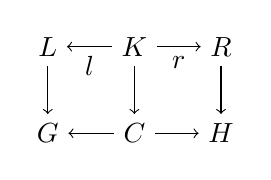
\begin{tikzpicture}[node distance=11mm]
          \node (I) {$K$};
          \node (L) [left of= I] {$L$};
          \node (R) [right of=I] {$R$}; 
          \node (G) [below of=L] {$G$};
          \node (C) [below of=I] {$C$};
          \node (H) [below of=R] {$H$};
        %   \node (T) [left=of $(L)!0.5!(G)$] {$T$};
        %   \draw [->] (L) to  node [label, above] {$c$}  (T);
        %   \draw [->] (G) to  node [label, below] {$\alpha$} (T);
          \draw [->] (I) to node [label, below] {$l$} (L);
          \draw [->] (I) to node [label, below] {$r$} (R);
          \draw [->] (L) to  (G);
          \draw [->] (I) to (C);
          \draw [->] (R) to (H);
          \draw [->] (C) to (G);
          \draw [->] (C) to (H);
        \end{tikzpicture}
      \end{center}
\end{minipage}
   \begin{itemize}
       \item $\operatorname{left}(\Delta)$ is weighable with \(\mathcal{T}\), and
       \item $\operatorname{right}(\Delta)$ is bounded above by \(\mathcal{T}\), and
       \item $w(e) \succeq 1_S$ for all $e \in \mathbb{E}$.
   \end{itemize}

   \noindent
  We have:
   \begin{itemize}
       \item $\mu(w_\mathcal{T}(G)) \succeq \mu(w_\mathcal{T}(H))$ if $\rho$ is weakly decreasing,
       \item $\mu(w_\mathcal{T}(G)) > \mu(w_\mathcal{T}(H)) + \delta$ if $\rho$ is $\delta$-uniformly or $\delta$-closure decreasing for some $\delta >0$ and $w(e) \succeq 1_S$ for all $e \in \mathbb{E}$.
   \end{itemize}
\end{lemma} 

\begin{proof}
    \label{proof:decreasing_step}
    \noindent For every \( t_K: K \rightarrow T \), we define
$
        S_{t_K} \overset{\operatorname{def}}{=}   
        \underset{\substack{t_C:C \rightarrow T \\
        t_K = h_{KC} \star t_C }}{\bigoplus} 
        w_\mathcal{T}(t_C - h_{KC})  
$.
    
    \noindent For all $t_K: K \to T$ and $X,Y \in S$, the following claims hold:
    \begin{enumerate}[label=(\alph*)] 
        \item \label{s_nz} $S_{t_K} \ne 0_S$ if there is $t_C$ with $ t_K = h_{KC} \star t_C$.  
        \begin{proof}
            By definition of weighted type graph, for all $e \in \mathbb{E}$, we have 
            \begin{flalign}
                w(e) \neq 0_S \label{eq_we_neq_0s1111}
            \end{flalign}
            For every $t_C:C \to T$, we have 
            \begin{flalign*}
                &w_\mathcal{T}(t_C - h_{KC}) \\
               =&\bigodot_{e\in \mathbb{E}} w_e(t_C - h_{KC}) & \text{by \autoref{def:weight_excluding}}\\
               =&\bigodot_{e\in \mathbb{E}} 
                 \bigodot_{\substack{\alpha \in \{- * t_C = e\}\\
                    \alpha \notin \left\{ \iota \in \operatorname{Hom}(X, C)~\middle|~\exists \zeta:X \to K,~\zeta \star h_{KC} = \iota \right\}
                 }
                 } w(e)  & \text{by \autoref{def:weight_excluding_pre}} \\
               \neq&0_S & \text{by \eqref{eq_we_neq_0s1111}, \eqref{eq:prop_neq0_mul_neq0} and \autoref{def:bigodot}}  
            \end{flalign*}

            Therefore, $S_{t_K} \overset{\operatorname{def}}{=}   
            \underset{\substack{t_C:C \rightarrow T \\
            t_K = h_{KC} \star t_C }}{\bigoplus} 
            w_\mathcal{T}(t_C - h_{KC}) \neq 0_S$ if there exists be a morphism such that $t_K = h_{KC} \star t_C$ by \eqref{eq:prop_neq0_plus_neq0}.
            % For every $t_C:C \to T$ such that $t_K = h_{KC} \star t_C$, we have $w_\mathcal{T}(t_C - h_{KC}) \neq 0_S$ by \eqref{eq:prop_neq0_mul_neq0}. 
        \end{proof}
        
        \item \label{s_ge1} $S_{t_K} \succeq 1_S$ if there is $t_C$ with $ t_K = h_{KC} \star t_C$ and $w_\mathcal{T}(e) \succeq 1_S$ for all $e \in \mathbb{E}$,
        \begin{proof}
            By the definition of weighted type graph, for all $e \in \mathbb{E}$, we have $w(e) \neq 0_S$.  
            By assumption, we have $w_\mathcal{T}(e) \succeq 1_S$ for all $e \in \mathbb{E}$. Thus, we have 
            \begin{flalign}
                1_S \preceq w(e) \neq 0_S \label{eq_we_neq_0s_geq1_0}
            \end{flalign}
            By \eqref{eq:prop_neg0_ge1_mul_ge1}, we have
            \begin{flalign}
                1_S \preceq w_\mathcal{T}(t_C - h_{KC}) \label{eq_we_neq_0s_geq1}
            \end{flalign}

            Therefore, $S_{t_K} \overset{\operatorname{def}}{=}   
            \underset{\substack{t_C:C \rightarrow T \\
            t_K = h_{KC} \star t_C }}{\bigoplus} 
            w_\mathcal{T}(t_C - h_{KC}) \succeq 1_S$ if there exists be a morphism such that $t_K = h_{KC} \star t_C$ by \eqref{ax:s1}.
        \end{proof}
        
        % \item \label{claim:le} $Y \succeq X \implies  Y \odot S_{t_K} \succeq X \odot S_{t_K}$
        % \\ by Axiom \eqref{ax:s3}. \todo{to delete: inutile}
         
        \item \label{claim:st} if there exists $t_C$ with $t_K = h_{KC} \star t_C$ then
        $$ \mu(Y) > \mu(X) + \delta  \implies \mu(Y \odot S_{t_K}) > \mu(X \odot S_{t_K})$$
                % $$\left (\exists \alpha \geq \delta.~\mu(Y) > \mu(X) + \alpha \right ) \implies (\mu(Y \odot S_{t_K}) > \mu(X \odot S_{t_K}))$$
        \begin{proof}
           Suppose that there is $t_C$ with $t_K = h_{KC} \star t_C$. We have $S_{t_K} \neq 0_S$ by \ref{s_nz}, and we conclude by \eqref{ax:s4''}.
        \end{proof}
    
        \item \label{claim:sh_{DT}elta} 
        if there exists $t_C$ with $t_K = h_{KC} \star t_C$, and  $w_\mathcal{T}(e) \succeq 1_S$ for all $e \in \mathbb{E}$ then
        % $$\left (\exists \alpha \geq \delta.~\mu(Y) > \mu(X) +  \alpha \right ) \implies (\exists \beta \geq \delta. \mu(Y \odot S_{t_K}) > \mu(X \odot S_{t_K})  + \beta)$$
        $$\mu(Y) > \mu(X) +  \delta \implies \mu(Y \odot S_{t_K}) > \mu(X \odot S_{t_K})  + \delta $$
        \begin{proof}
            Suppose that there is $t_C$ with $t_K = h_{KC} \star t_C$. We have $1_S \preceq S_{t_K} \neq 0_S$ by \ref{s_nz} and \ref{s_ge1}, and we conclude by \eqref{ax:s4'}. 
        \end{proof}

        \item \label{claim:0} 
        if there is no $t_C$ with $t_K = h_{KC} \star t_C$ then  $S_{t_K} = 0_S$, thus
        $$Y \odot S_{t_K} = 0_S = X \odot S_{t_K} $$
    
        \item \label{claim:exist_st} 
        If there is a context closure $t_L$ for $\rho$ and $T$ in $\mathfrak{F}$ , then, let $t_K = l \star t_L$, we have
        $$ \mu(Y) > \mu(X) + \delta \implies \mu(Y \odot S_{t_K}) > \mu(X \odot S_{t_K})$$
        \begin{proof}
            
       By \autoref{def:context_closure} of context closure, there exists $t_G : G \rightarrow T$ such that 
        \begin{flalign*}
             t_L = h_{LG} \star t_G \tag{1} \label{eq_tl_hlg_tg}
        \end{flalign*}
      i.e. we have the following commutative diagram
     
    \begin{center}
        \begin{tikzpicture}[node distance=11mm]
          \node (I) {$K$};
          \node (L) [left of= I] {$L$};
          \node (R) [right of=I] {$R$};
          \node (G) [below of=L] {$G$};
          \node (C) [below of=I] {$C$};
          \node (H) [below of=R] {$H$};
          \node (T) [left=of $(L)!0.5!(G)$] {$T$};
          \draw [->] (L) to  node [label, above] {$t_L$}  (T);
          \draw [->] (G) to  node [label, below] {$t_G$} (T);
          \draw [->] (I) to node [label, above] {$l$} (L);
          \draw [->] (I) to node [label,above] {$r$} (R);
        %   \draw [->] (L) to node [label, right] {$m$} (G);
        \draw [->] (L) to node [label, right] {} (G);
          \draw [->] (I) to (C);
          \draw [->] (R) to (H);
          \draw [->] (C) to (G);
          \draw [->] (C) to (H);
        \end{tikzpicture}
      \end{center}
    
        Let $t_C \overset{\operatorname{def}}{=} h_{CG} \star t_G$ and $t_K \overset{\operatorname{def}}{=} l \star t_L$. We have\\
        \begin{flalign*}
              t_K  &=  l \star t_L &\text{by definition of $t_K$}
            \\ &=   l \star (h_{LG}  \star t_G) & \text{by \autoref{eq_tl_hlg_tg}}
            \\ &= (l \star h_{LG}) \star t_G &\text{by associativity }
            \\ &= (h_{KC} \star h_{CG}) \star t_G & \text{by commutative of $\square KLGC$}
            \\ &= h_{KC} \star (h_{CG}  \star t_G) & \text{by associativity}
            \\ & = h_{KC} \star t_C &\text{by definition of $t_C$}
        \end{flalign*}
        and the claim follows from \ref{claim:st}, sinc $t_C$ is a morphism such that $t_K = h_{KC} \star t_C$.
    \end{proof}

        \item \label{claim:exist_sh_{DT}elta} 
        If there is a context closure $t_L$ for $\rho$ and $T$ in $\mathfrak{F}$, and $w_\mathcal{T}(e) \succeq 1_S$ for all $e \in \mathbb{E}$ then, let $t_K = l \star t_L$, we have 
            % $$\left (\exists \alpha \geq \delta. Y \succ X +  \alpha \right ) \implies (\exists \beta \geq \delta. Y \odot S_{t_K} \succ X \odot S_{t_K}  + \beta)$$
        $$Y \succ X + \delta \implies Y \odot S_{t_K} \succ X \odot S_{t_K}  + \delta$$ 
        \begin{proof}
            The proof is analogous to the proof of \ref{claim:exist_st} but with \ref{claim:sh_{DT}elta} instead of \ref{claim:st} in the end.
        \end{proof} 
    \end{enumerate}
    
    \noindent For every \( t_K: K \rightarrow T \), let
    \begin{flalign*}
        \Lambda_{t_K} &\overset{\operatorname{def}}{=}  w_\mathcal{T}(\{l \star - = t_K\})
        \\
        \Omega_{t_K} &\overset{\operatorname{def}}{=}  w_\mathcal{T}(\{r \star - = t_K\})
    \end{flalign*}
  By \autoref{lem_4d13}, we have 
        \begin{flalign*} 
            w_\mathcal{T}(G) &=
                \underset{\substack{t_K: K \rightarrow T}}{\bigoplus}     \ \
            (S_{t_K} \odot \Lambda_{t_K})
              \\
            w_\mathcal{T}(H) &\preceq
            \underset{\substack{t_K: K \rightarrow T}}{\bigoplus}     \ \
                (S_{t_K} \odot \Omega_{t_K})
        \end{flalign*}

    \noindent We complete the proof with a analysis by cases:
    \begin{enumerate}
        \item  If $\rho$ is weakly decreasing, then, by \autoref{def:decreasing_rule} of weakly decreasing rule, we have $\Lambda_{t_K} \geq \Omega_{t_K}$
        for every $t_K: K \rightarrow T$. 
        By \eqref{ax:s3}, for every  $ t_K : K \rightarrow T$, we have 
                \begin{flalign*} 
                    S_{t_K} \odot \Lambda_{t_K} \succeq S_{t_K} \odot \Omega_{t_K} \tag{NE} \label{steps:weightC:ge} 
                \end{flalign*}
        Thus, we have $w_\mathcal{T}(G) \succeq w_\mathcal{T}(H)$, from \eqref {ax:s1}.
        % \item
        %     If $\rho$ is $\delta$-uniformly decreasing for some $\delta \in \mathbb{R}_{>0}$, then, by \autoref{def:decreasing_rule} of $\delta$-uniformly decreasing rule,
        %     for all $t_K : K \to T$, we have 
        %                     \begin{itemize}                                
        %                         \item $\exists \alpha \geq \delta.~\mu(\Lambda_{t_K}) > \mu(\Omega_{t_K}) + \alpha$, or
        %                         \item $\{l \star - = t_K\} = \emptyset = \{r \star - = t_K\}$
        %                     \end{itemize}
        %     From \ref{claim:st} and \ref{claim:0}, for every \( t_K: K \rightarrow T \), we have
        %     \begin{enumerate}[label=(\roman*)]
        %         \item $S_{t_K} \odot \Lambda_{t_K} = 0_S =  S_{t_K} \odot \Omega_{t_K}$, or        
        %         \item  \label{it:strict} $ \mu(\Lambda_{t_K} \odot S_{t_K}) >  \mu(S_{t_K} \odot \Omega_{t_K})$
        %     \end{enumerate}
        %     To establish $ \mu(w_\mathcal{T}(G)) > \mu(w_\mathcal{T}(H))$, using \eqref{ax:s2}, 
        %     it suffices to show that we have case~\ref{it:strict} for some $t_K : K \to T$.
        %     This follows from \ref{claim:exist_st} since we have a context closure for $\rho$ and $\mathcal{T}$, by assumption.
        \item  
            Suppose that $\rho$ is $\delta$-uniformly decreasing for $\delta \in \mathbb{R}_{>0}$, and $w_\mathcal{T}(e) \succeq 1$ for all $e \in \mathbb{E}$. By \autoref{def:decreasing_rule} of $\delta$-uniformly decreasing rule,
            for all $t_K : K \to T$, we have  
                            \begin{itemize}                                
                                \item $\mu(\Lambda_{t_K}) > \mu(\Omega_{t_K}) + \delta$,
                                % $\exists \alpha \geq \delta  .~\mu(\Lambda_{t_K}) > \mu(\Omega_{t_K}) + \alpha$, 
                                 or
                                \item $\{l \star - = t_K\} = \emptyset = \{r \star - = t_K\}$
                            \end{itemize}
            From \ref{claim:sh_{DT}elta} and \ref{claim:0}, for every \( t_K: K \rightarrow T \), we obtain
            \begin{enumerate}[label=(\roman*)]
                \item $S_{t_K} \odot \Lambda_{t_K} = 0_S =  S_{t_K} \odot \Omega_{t_K}$, or
                \item  \label{it:strich_{DT}elta}  $\mu(\Lambda_{t_K} \odot S_{t_K}) > \mu(\Omega_{t_K} \odot S_{t_K}) + \delta$
                % $\exists \beta \geq \delta  .\  \mu(\Lambda_{t_K} \odot S_{t_K}) > \mu(\Omega_{t_K} \odot S_{t_K}) + \beta$
            \end{enumerate}
            To establish $ \mu(w_\mathcal{T}(G)) > \mu(w_\mathcal{T}(H)) + \delta$, using \eqref{ax:s2'}, 
            it suffices to show that we have case~\ref{it:strich_{DT}elta} for some $t_K : K \to T$.
            This follows from \ref{claim:exist_sh_{DT}elta} since we have a context closure for $\rho$ and $\mathcal{T}$ by assumption.
            % \item
            % If $\rho$ is $\delta$-closure decreasing, 
            % then it is also weakly decreasing and we obtain \eqref{steps:weightC:ge} for every $t_K : K \to T$.
            % Since the semiring is strictly ordered museurable, it suffices to show that there exists some $t_K : K \to T$ such that
            % \begin{align}
            %    \mu( S_{t_K} \odot \Lambda_{t_K})  \succ \mu(S_{t_K} \odot \Omega_{t_K})
            %   \tag{$\star$} \label{steps:weightC:gt}
            % \end{align}
            % in order to conclude $\mu(w_\mathcal{T}(G)) > \mu(w_\mathcal{T}(H))$ by~\eqref{ax:s5}.
            % By \autoref{def:decreasing_rule}, there is a context closure $t_L$ for $\rho$ and $T$, and 
            % % $\exists \delta' \geq \delta  .\  \Lambda_{t_K} > \Omega_{t_K} + \delta'$
            % $\mu(\Lambda_{t_K}) > \mu(\Omega_{t_K}) + \delta$
            % for $t_K = l \star t_L$. Thus, we obtain ~\eqref{steps:weightC:gt} by~\ref{claim:exist_st}.
        \item
            If $\rho$ is $\delta$-closure decreasing, and $w_\mathcal{T}(e) \succeq 1$ for all $e \in \mathbb{E}$ then it is also weakly decreasing and we obtain \eqref{steps:weightC:ge} for every $t_K : K \to T$.
            Since the semiring is a strictly monotonic museurable semiring,  by~\autoref{ax:s2'} and \eqref{ax:s5'}, it suffices to show that there exists some $t_K : K \to T$ such that 
            \begin{align}
                % \exists \alpha \geq \delta.~
                \mu(S_{t_K} \odot \Lambda_{t_K}) > \mu(S_{t_K} \odot \Omega_{t_K}) + 
                \delta
                % \alpha
              \tag{$\star\star$}\label{steps:weightC:gh_{DT}elta}
            \end{align}
            in order to conclude $ \mu(w_\mathcal{T}(G)) > \mu(w_\mathcal{T}(H)) + \delta$.
            There is a context closure $t_L$ for $\rho$ and $T$, and
            $\mu(\Lambda_{t_K}) > \mu(\Omega_{t_K}) + \delta$
            % $\exists \delta' \geq \delta  .\  \Lambda_{t_K} > \Omega_{t_K} + \delta'$
            for $t_K = l \star t_L$. Thus, we obtain~\eqref{steps:weightC:gh_{DT}elta} by~\ref{claim:exist_sh_{DT}elta}.
    \end{enumerate}
    % \qed
\end{proof} 

\subsection{Termination Criterion}
\label{sec:nwf:proving_termination}
Finally, we formulate a termination criterion leveraging type graphs weighted over non-well-founded semirings. 
\begin{theorem}[Termination of DPO rewriting system] 
    \label{thm:termination_grs}
    Let $\mathcal{A}$ and $\mathcal{B}$ be sets of DPO rewriting rules, $\mathcal{T} = (T,\mathbb{E}, (S, \oplus, \odot, 0_S, 1_S, \prec, \mu), w)$ a finitary weighted type graph and $\mathfrak{F}$ a DPO rewriting framework such that

     \begin{enumerate}[label=\roman*)]
        \item\label{thm1:hyp3} $w(e) \succeq 1_S$ for all $e \in \mathbb{E}$, and
        % \item\label{thm1:hyp4} $\{s \in S\mid 1_S \leq s \neq 0_S\} \subseteq \mathbb{R}_{>0}$ 
        % \item\label{thm1:hyp4} for all $x \in S$, if $ 1_S \preceq x \neq 0_S$ then $\mu(x) \geq \mu(1_S)$ and $\mu(x) \in \mathbb{R}$,
        \item\label{thm1:hyp4} for all $x \in S$, if $ 1_S \preceq x \neq 0_S$ then $\mu(x) \geq \mu(1_S)$ and $\mu(x) \in \mathbb{R}$, and
        \item for every rule $\rho \in (\mathcal{A }\cup \mathcal{B })$ and every double pushout diagram  
        $\Delta \in \mathfrak{F}(\rho)$ 
        \begin{itemize}
            \item \(\operatorname{left}(\Delta)\) is weighable with \(\mathcal{T}\),
            \item \(\operatorname{right}(\Delta)\) is bounded above by \(\mathcal{T}\). 
        \end{itemize}
    \end{enumerate}       

    \noindent If the following conditions hold:
    \begin{enumerate}
        \item there exists $\delta >0$ such that either every $\rho \in \mathcal{A}$ is $\delta$-uniformly decreasing, or every $\rho \in \mathcal{A}$ is $\delta$-closure decreasing, and
        \item every rule $\rho \in \mathcal{B}$ is weakly decreasing,
    \end{enumerate}
    then $\Rightarrow_{\mathcal{A},\mathfrak{F}}$ is \textbf{terminating} relative to $\Rightarrow_{\mathcal{B},\mathfrak{F}}$.
\end{theorem} 
% \begin{proof}
%     See the \hyperref[proof_termination_grs]{Appendix}.
% \end{proof}

\begin{proof} 
    \label{proof_termination_grs}
    From the definition of weighted type graph, we have 
    $$\text{for all}~e\in\mathbb{E}, w(e) \neq 0_S$$ 
    From ssumption \eqref{thm1:hyp3}, we have 
    $$\text{for all}~e\in\mathbb{E},1_S \preceq w(e)$$
    Therefore, we have 
    \begin{flalign}
        \text{for all}~e\in\mathbb{E},1_S \preceq w(e)\neq 0_S \label{thm_eq_we_neq0_geq1}
    \end{flalign} 
    Let $G$ be a graph admitting a match of a DPO rewriting rule. We have 
    \begin{flalign*}
        w_\mathcal{T}(G) &\overset{\operatorname{def}}{=} 
            \underset{h \in \operatorname{Hom}(G,T)}{\bigoplus}  w_\mathcal{T}(h) \\
        & \overset{\operatorname{def}}{=} 
        \underset{h \in \operatorname{Hom}(G,T)}{\bigoplus} 
            \left ( \underset{e \in \mathbb{E}}{\bigodot} 
            \left(  
                \underset{\alpha \in \{- \star h = e\}}{\bigodot}w(e) 
            \right)
            \right )\\
    \end{flalign*} 
    By \autoref{thm_eq_we_neq0_geq1}, \autoref{prop_endrullis_2d7}, {def:bigodot} and $1_S \neq 0_S$, for every $h \in \operatorname{Hom}(G,T)$, we have
    \begin{flalign}
        1_S \preceq 
        \underset{e \in \mathbb{E}}{\bigodot} 
                \left(  
                    \underset{\alpha \in \{- \star h = e\}}{\bigodot}w(e) 
                \right) 
        \neq 0_S
    \end{flalign}
    Since $G$ be a graph admitting a match of a DPO rewriting rule, by \autoref{prop_endrullis_2d7} and \eqref{ax:s0}, we have $$1_S \preceq w_\mathcal{T}(G) \neq 0_S$$
    % By \autoref{prop_endrullis_2d7} and \eqref{ax:s0}, we have 
    % $$\forall G\in\mathcal{C}_0, (\exists H\in \mathcal{C}_0. G \Rightarrow_\mathcal{R} H) \rightarrow (1_S \preceq w_\mathcal{T}(G) \neq 0_S)$$
    By Assumption \eqref{thm1:hyp4}, we have 
    % $$\forall G\in\mathcal{C}_0, (\exists H\in \mathcal{C}_0. G \Rightarrow_\mathcal{R} H) \rightarrow (\mu(w_\mathcal{T}(G)) \geq \mu(1_S))$$
      $$\mu(w_\mathcal{T}(G)) \geq \mu(1_S)$$
 
    % Let $G \in \mathcal{C}_0$ be an object. By Assumption \ref{thm1:hyp4}, we have $\mu(w_\mathcal{T}(G)) \in \mathbb{R}$ and $\mu(w_\mathcal{T}(G)) \geq \mu(1_S)$.

    By \autoref{lem:decreasing_step}, every rewriting step with rules in $\mathcal{A}$ strictly decreases the weight by at least $\delta$ and no rewriting step with rules in $\mathcal{B}$ increases the weight.
    Consequently, there is no infinite rewriting sequence with an infinite rewriting steps with rules in $\mathcal{A}$ from $G$.
\end{proof}
\begin{example}
    \label{example:termination}
    Termination of the DPO rule in \autoref{ex:grsaa} can be established using \autoref{thm:termination_grs} together with the weighted type graph in \autoref{example:weighted_type_graph} over the real arithmetic semiring $\mathfrak{N}' = (\mathbb{R}^+,+,*,0_\mathbb{R},1_\mathbb{R},<,\operatorname{id}_{\mathbb{R}^+})$. It is $\delta$-closure decreasing with $\delta = 0.5$ by \autoref{example:decreasing_rule}.
\end{example}

